%==============================================================================
\chapter{Datasets and Event Selection}
\label{sec:Samples}
%==============================================================================
This chapter introduces the datasets uses for the Neural Network studies carried out in the following chapters. An overview of the steps taken to simulate the different background and signal datasets is given as well as a short introduction of event weights. The chapter is then concluded by the description of the event selection and the definition of the signal region.

\section{Simulated Datasets}
\label{sec:Simulation}
The data used in this thesis does not come from real proton-proton collisions measured in the ATLAS detector but rather is simulated data. These simulations are essential to accurately estimate the underlying background and for optimal signal selection. The ATLAS simulation chain \cite{ATLASsim} can be divided into three steps: generation of the event and immediate hadronization and decay of the produced particles, simulation of the particle interaction with the detector such as parton showering,  and digitization of the detector responses into voltages and currents. The event generation can proceed at different levels of precision. A leading-order (LO) event generation only takes those production processes into account that have the smallest power of the coupling constant among all possible contributing processes. On the other hand, a next-to-leading-order (NLO) calculation additionally considers production processes which are sub-leading in the coupling constant power.  \\
The datasets used for the signal and all backgrounds are simulated to match the full Run 2 dataset. It consists of three sub-campaigns MC16a corresponding to the data taking conditions in the years 2015 and 2016, MC16d for the year 2017, and MC16e for the year 2018. The $t\bar{t}t\bar{t}$ events are simulated using {\scshape MadGraph5\_Amc@NLO} \cite{MadGraph} at NLO precision. The top quarks are decayed at LO using {\scshape MadSPIN} whereas the parton showers and hadronization processes are modeled by {\scshape Pythia8}\cite{PYTHIA}. In addition to the first NLO $t\bar{t}t\bar{t}$ dataset, a second signal dataset produced at LO precision is available. \\
The background datasets are summarized in table \ref{tab:generatros} together with the used event generators and parton shower simulation programs. All backgrounds expect $t\bar{t}$+Diboson and $V$+jets\footnote{$V$ corresponds to either a W or a Z boson} are produced at NLO precision. $t\bar{t}$+Diboson was generated at LO but scaled the NLO cross-section. $V$+jets is simulated at NLO for up to two jets and at LO for up to four jets. The dataset referred to as ``others'' mainly contains $t\bar{t}t$ events but also $VH$ and $VVV$ events. More details about the datasets can be found in the official ATLAS four-top-quark analysis \cite{cross5}. The final simulation step of the ATLAS detector responses to the different final state particles is modeled by {\scshape AltFast} \uproman{2} \cite{AltFast}. \\
An additional dataset containing $t\bar{t}t\bar{t}$ and $t\bar{t}t$ events was simulated (MC16e only) for reconstruction studies and will not be used as an additional background in the $t\bar{t}t\bar{t}$ analysis. Similar to all other samples it contains information about reconstructed objects. Additionally, information not available at reconstruction level called \textit{truth information} is available for this dataset. An example for truth information would be the information if a W boson decays hadronically or leptonically. The $t\bar{t}t$ events are generated by {\scshape MadGraph5\_Amc@NLO} while the parton showering is simulated using {\scshape PYTHIA8}. 

\begin{table}[H]
\centering
\begin{tabular}{|r|r|r|}
\toprule
Dataset & Event generator & parton showering \\
\midrule
\midrule
$t\bar{t}t\bar{t}$ & \scshape MadGraph5\_Amc@NLO & \scshape PYTHIA8 \\
$t\bar{t}W$ & \scshape Sherpa \cite{Sherpa} & \scshape Sherpa \\
$t\bar{t}WW$ & \scshape MadGraph5\_Amc@NLO & \scshape PYTHIA8 \\
$t\bar{t}Z$ & \scshape MadGraph5\_Amc@NLO & \scshape PYTHIA8 \\
$t\bar{t}H$ & \scshape PowHegBox \cite{PowHeg} & \scshape PYTHIA8 \\
$t\bar{t}$ & \scshape PowHegBox & \scshape PYTHIA8 \\
$t(\bar{t})X$ & \scshape PowHegBox & \scshape PYTHIA8 \\
$V$+jets & \scshape Sherpa & \scshape Sherpa \\
$VV$ & \scshape Sherpa & \scshape Sherpa \\
others & MadGraph5\_Amc@NLO & \scshape PYTHIA8 \\
$t\bar{t}t$ & \scshape MadGraph5\_Amc@NLO & \scshape PYTHIA8 \\
\bottomrule
\end{tabular}
\caption{Summary of the event generator and parton showering programs used for the different datasets.}
\label{tab:generatros}
\end{table}

\paragraph{Event Weights} \mbox{} \\

The datasets described above contain combined $\sim 2700000$ events that pass the preselection which will be introduced in the next section. The $t\bar{t}W$ datasets contains $\sim 400000$ events while the NLO $t\bar{t}t\bar{t}$ dataset contains $\sim 500000$ events. However, the cross-section of the $t\bar{t}W$ at 13TeV is an order of magnitude larger than the cross section of four-top-quark events and even after applying the preselection the ratio is still approximately 20 (c.f. Figure \ref{fig:HT_preselection}). The number of generated data events $N_{\text{gen}}$ for each process can be scaled to the number of events measured in the detector and passing all preselections $N_{\text{pass}}$ by applying Luminosity weights $w _{\text{Lumi}}$ defined by
\begin{equation}
\label{eq:weights}
w _{\text{Lumi}} = \frac{N_{\text{exp}}}{N_{\text{pass}}} = \frac{\sigma \cdot L}{N_{\text{gen}}}
\end{equation}
which directly follow from Equation \ref{eq:Lumi} by expressing $\epsilon$ as $\frac{N_{\text{pass}}}{N_{\text{gen}}}$. Moreover, different event by event weights have to be applied to account for different beam and detector configurations such as pile up, lepton scaling factor, jet vertex tagger, and b-tagging scaling factor weights. A special weight is the generator weight \cite{PDG2020}, originating from the evaluation of the phase space integral during the generation of the events. For next to leading order event generation this weight can become negative due to the calculation contribution of loop amplitudes \cite{nWeights} which often can be problematic for machine learning methods. The effective number of observable events after applying the weight sum will be referred to as event \textit{Yield}.

\section{Object and Event Selection}
\label{sec:EventSelection}

The signal and background datasets contain four different reconstructed objects electrons, muons, jets, b-jets and $E_{\text{T}}^{miss}$. An overlap removal procedure depending on the distance between two objects is applied to ensure that calorimeter clusters and particle tracks are not signed twice to different objects. \\
The event preselection will be defined in the following. Events passing the preselection have to have fired a single-lepton or dilepton trigger. The $p_{\text{T}}$ threshold of these triggers vary depending on the fulfilled isolation requirements of the leptons and the data-taking period. Only those events which have at least one vertex reconstructed from at least two inner detector tracks with transverse momenta of $p_{\text{T}}>\SI{0.4}{GeV}$ are considered. The kinematic preselection requirements for leptons and jets are summarized in Table \ref{tab:requirements}. Additionally, the electron charge identification selector (ECIDS) \cite{ECIDS} is applied for final states with two electron or an electron and a muon. The ECIDS suppress the charge misidentification background significantly. Jets are reconstructed using the anti-k$_{t}$ algorithm \cite{Akt} (R = 0.4). To reduce pile-up, jets are furthermore required to have a transverse momentum of $p_{\text{T}}$ and $|\eta| < 2.4$. B-jets are identified using a multivariate algorithm called MV2c10 \cite{MV2c10} , where c10 refers to the fact that 10\% of the background dataset are c-jets. The pseudo-continuous working points provided are 80\%, 77\%, 70\%, and 60\% b-tagging efficiency. The working point selected for this analysis is 77\% b-tagging efficiency.
 
\begin{table}[H]
\centering
\begin{tabular}{|r|r|r|}
\toprule
Particle type & $p_{\text{T}}$ & $|\eta|$ \\
\midrule
\midrule
Electrons & $> \SI{28}{GeV}$ & $<2.47$ \\
Muons & $> \SI{28}{GeV}$ & $<2.5$ \\
Jets & $> \SI{25}{GeV}$ & $<2.5$ \\
B-jets & $> \SI{28}{GeV}$ & $<2.5$ \\
\bottomrule
\end{tabular}
\caption{Transverse momentum and pseudorapidity preselections for the different particles, the crack region is excluded.}
\label{tab:requirements}
\end{table}


\paragraph{Signal Region} \mbox{} \\

Events entering the signal region come from the Same Sign Multi-Lepton channel SSML where two same-sign leptons or at least three leptons are required. The branching fraction of this channel is $BR = 0.12$ (cf. Table \ref{tab:fourtopdecays}) where the biggest contribution originates from the same signed lepton events $BR = 0.07$. The definition of the signal region is then completed by requiring at least 6 jets among which are at least two b-tagged as well as a scalar sum of all lepton and jet $p_{\text{T}}$'s $H_{\text{T}}$ high than $\SI{500}{GeV}$.   \\
Figure \ref{fig:HTSR} shows the $H_{\text{T}}$ distributions before the definition of the signal region is applied (a) and after (b). As can be seen, the amount of background events is significantly decreased in the signal region. To quantify this observation the \textit{signal efficiency} $s$ is defined as
\begin{equation}
\label{eq:sigeff}
s = \frac{Y_s}{\sqrt{Y_s + Y_b}}
\end{equation}
where $Y_s$ and $Y_b$ are the signal and background Yield. The calculated values for the signal efficiency after allying the requirements of the signal region and before are 0.8 and 1.8. The total number of events available for training Neural Networks, introduced in Chapter \ref{sec:Deep_learning}, decreases to $\sim 700000$ events. The number of events fulfilling the preselection and in of the signal region are summarized in Table \ref{tab:prevssr} in the Appendix. The dominant backgrounds in the signal region are $t\bar{t}W$, $t\bar{t}Z$ and $t\bar{t}H$. The backgrounds coming from $t\bar{t}X$ are split depending on the instrumental effects and physics processes that lead to a final state similar to that of $t\bar{t}t\bar{t}$ event:
\begin{enumerate}[leftmargin=2cm]
\item[QmisID:] events with one lepton having its charge mis-identified
\item[CO:] events with one lepton coming from photon material conversion
\item[HF:] events with one lepton coming from heavy-flavour meson decay
\item[light:] events with one lepton coming from light-meson decay or events with one wrongly identified jet as a lepton
\item[other:] events falling into none of the above categories
\end{enumerate}
Minor backgrounds are diboson production $VV$, associated production of bosons with jets $V$+jets, single top $t(\bar{t})X$ and $t\bar{t}WW$ as well as the previously introduced datasets of ``others''.


\begin{figure}[H]
\begin{subfigure}{\textwidth}
  \centering
  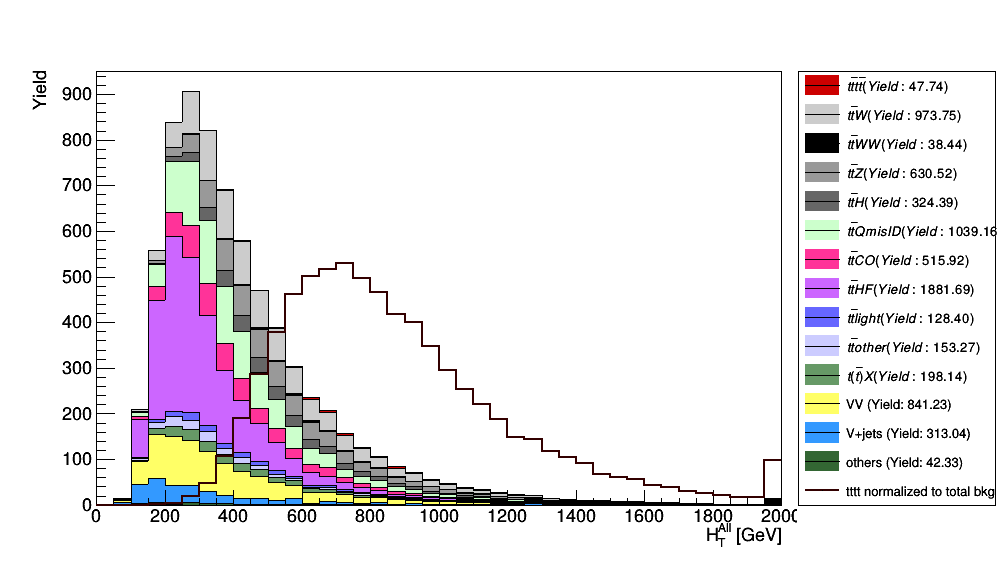
\includegraphics[width=.95\linewidth]{figs/HT_presection.png}
  \caption{Preselection}
  \label{fig:HT_preselection}
\end{subfigure} \\
\begin{subfigure}{\textwidth}
  \centering
  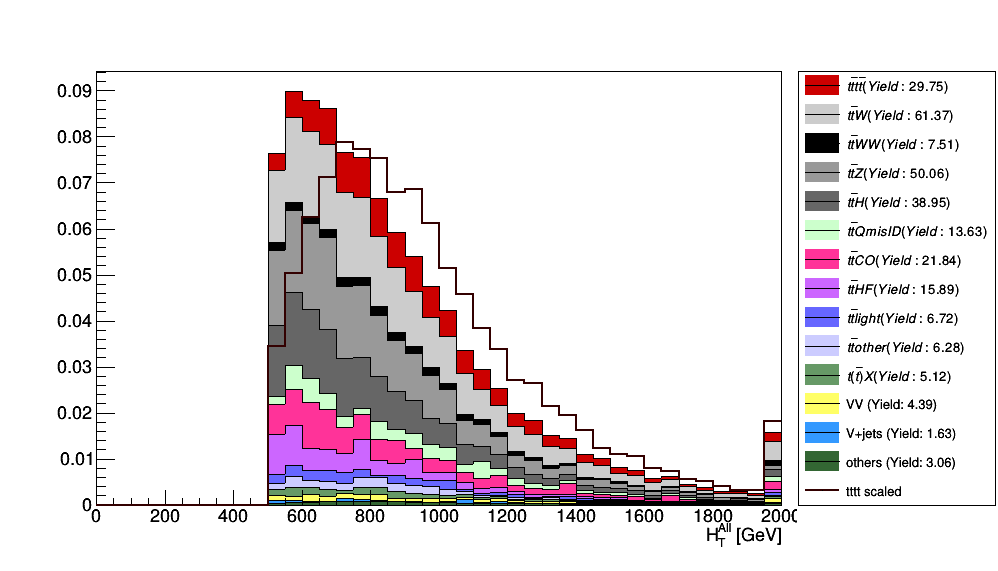
\includegraphics[width=.95\linewidth]{figs/HT_sr.png}
  \caption{Signal Region}
  \label{fig:HT_sr}
\end{subfigure}
\caption{Sum of the transverse momentum of all leptons and jets ($H_{\text{T}}$) after applying the preselection (a) and in the signal region (b). The dark red line shows the signal scaled to the total background yield. The last bin contains additionally all events with $H_{\text{T}} > 2000$}
\label{fig:HTSR}
\end{figure}